\documentclass[11pt]{article}
\usepackage[margin=1in]{geometry}
\usepackage[T1]{fontenc}
\usepackage{lmodern}
\usepackage{microtype}
\usepackage{amsmath}
\usepackage{booktabs}
\usepackage{graphicx}
\usepackage{xcolor}
\usepackage[numbers,sort&compress]{natbib}
\usepackage[hidelinks]{hyperref}
\usepackage{caption}
\captionsetup{font=small,labelfont=bf}
\graphicspath{{../figures/}}

% Generated by pipeline/report.py. Do not edit.
\newcommand{\ArbHours}{6,009}
\newcommand{\ArbDays}{549}
\newcommand{\ArbFirst}{2024-07-01}
\newcommand{\ArbLast}{2025-12-31}
\newcommand{\ArbDcKw}{893}
\newcommand{\ArbAcKw}{662.4}
\newcommand{\ArbPersNrmse}{0.209}
\newcommand{\ArbPersNmae}{0.120}
\newcommand{\ArbPersBias}{+0.001}
\newcommand{\ArbPersSkill}{-0.07}
\newcommand{\ArbPersLo}{-0.10}
\newcommand{\ArbPersHi}{-0.05}
\newcommand{\ArbPersSkillCommon}{-0.10}
\newcommand{\ArbSmartNrmse}{0.194}
\newcommand{\ArbSmartNmae}{0.122}
\newcommand{\ArbSmartBias}{-0.003}
\newcommand{\ArbPhysNrmse}{0.179}
\newcommand{\ArbPhysNmae}{0.123}
\newcommand{\ArbPhysBias}{+0.071}
\newcommand{\ArbPhysSkill}{+0.08}
\newcommand{\ArbPhysLo}{+0.00}
\newcommand{\ArbPhysHi}{+0.15}
\newcommand{\ArbPhysSkillCommon}{+0.17}
\newcommand{\ArbPhysCalNrmse}{0.158}
\newcommand{\ArbPhysCalNmae}{0.108}
\newcommand{\ArbPhysCalBias}{+0.035}
\newcommand{\ArbPhysCalSkill}{+0.19}
\newcommand{\ArbPhysCalLo}{+0.13}
\newcommand{\ArbPhysCalHi}{+0.24}
\newcommand{\ArbPhysCalSkillCommon}{+0.22}
\newcommand{\ArbGbmNrmse}{0.147}
\newcommand{\ArbGbmNmae}{0.096}
\newcommand{\ArbGbmBias}{+0.029}
\newcommand{\ArbGbmSkill}{+0.25}
\newcommand{\ArbGbmLo}{+0.20}
\newcommand{\ArbGbmHi}{+0.29}
\newcommand{\ArbGbmSkillCommon}{+0.27}
\newcommand{\ArbPhysEcNrmse}{0.160}
\newcommand{\ArbPhysEcNmae}{0.109}
\newcommand{\ArbPhysEcBias}{+0.059}
\newcommand{\ArbPhysEcSkill}{+0.18}
\newcommand{\ArbPhysEcLo}{+0.07}
\newcommand{\ArbPhysEcHi}{+0.27}
\newcommand{\ArbPhysEcSkillCommon}{+0.32}
\newcommand{\ArbPhysCalEcNrmse}{0.152}
\newcommand{\ArbPhysCalEcNmae}{0.104}
\newcommand{\ArbPhysCalEcBias}{+0.039}
\newcommand{\ArbPhysCalEcSkill}{+0.22}
\newcommand{\ArbPhysCalEcLo}{+0.13}
\newcommand{\ArbPhysCalEcHi}{+0.30}
\newcommand{\ArbPhysCalEcSkillCommon}{+0.32}
\newcommand{\ArbGbmEcNrmse}{0.144}
\newcommand{\ArbGbmEcNmae}{0.092}
\newcommand{\ArbGbmEcBias}{+0.029}
\newcommand{\ArbGbmEcSkill}{+0.26}
\newcommand{\ArbGbmEcLo}{+0.18}
\newcommand{\ArbGbmEcHi}{+0.33}
\newcommand{\ArbGbmEcSkillCommon}{+0.34}
\newcommand{\ArbPhysEraNrmse}{0.166}
\newcommand{\ArbPhysEraNmae}{0.111}
\newcommand{\ArbPhysEraBias}{+0.061}
\newcommand{\ArbPhysEraSkill}{+0.15}
\newcommand{\ArbPhysEraLo}{+0.04}
\newcommand{\ArbPhysEraHi}{+0.25}
\newcommand{\ArbPhysEraSkillCommon}{+0.30}
\newcommand{\ArbPhysCalEraNrmse}{0.155}
\newcommand{\ArbPhysCalEraNmae}{0.106}
\newcommand{\ArbPhysCalEraBias}{+0.044}
\newcommand{\ArbPhysCalEraSkill}{+0.20}
\newcommand{\ArbPhysCalEraLo}{+0.11}
\newcommand{\ArbPhysCalEraHi}{+0.29}
\newcommand{\ArbPhysCalEraSkillCommon}{+0.30}
\newcommand{\ArbGbmEraNrmse}{0.144}
\newcommand{\ArbGbmEraNmae}{0.091}
\newcommand{\ArbGbmEraBias}{+0.033}
\newcommand{\ArbGbmEraSkill}{+0.26}
\newcommand{\ArbGbmEraLo}{+0.16}
\newcommand{\ArbGbmEraHi}{+0.34}
\newcommand{\ArbGbmEraSkillCommon}{+0.36}
\newcommand{\ArbTransferNrmse}{0.175}
\newcommand{\ArbTransferNmae}{0.133}
\newcommand{\ArbTransferBias}{+0.039}
\newcommand{\ArbTransferSkill}{+0.10}
\newcommand{\ArbTransferLo}{+0.03}
\newcommand{\ArbTransferHi}{+0.16}
\newcommand{\ArbTransferSkillCommon}{+0.14}
\newcommand{\ArbSmartNrmseCommon}{0.204}
\newcommand{\ArbDaysCommon}{304}
\newcommand{\ArbCovGfs}{59}
\newcommand{\ArbWidthGfs}{0.209}
\newcommand{\ArbPinballGfs}{0.0310}
\newcommand{\ArbGainLoGfs}{-0.018}
\newcommand{\ArbGainHiGfs}{-0.005}
\newcommand{\ArbCovEc}{56}
\newcommand{\ArbWidthEc}{0.178}
\newcommand{\ArbPinballEc}{0.0307}
\newcommand{\ArbGainLoEc}{-0.016}
\newcommand{\ArbGainHiEc}{-0.001}
\newcommand{\ArbCovEra}{54}
\newcommand{\ArbWidthEra}{0.175}
\newcommand{\ArbPinballEra}{0.0308}
\newcommand{\ArbGainLoEra}{-0.020}
\newcommand{\ArbGainHiEra}{-0.003}
\newcommand{\ArbTransferGapLo}{-0.036}
\newcommand{\ArbTransferGapHi}{-0.020}
\newcommand{\ArbClearDays}{343}
\newcommand{\ArbClearGbmNrmse}{0.103}
\newcommand{\ArbClearSmartNrmse}{0.170}
\newcommand{\ArbClearGbmSkill}{+0.40}
\newcommand{\ArbClearPhysCalSkill}{+0.34}
\newcommand{\ArbMixedDays}{138}
\newcommand{\ArbMixedGbmNrmse}{0.181}
\newcommand{\ArbMixedSmartNrmse}{0.211}
\newcommand{\ArbMixedGbmSkill}{+0.14}
\newcommand{\ArbMixedPhysCalSkill}{+0.03}
\newcommand{\ArbOvercastDays}{68}
\newcommand{\ArbOvercastGbmNrmse}{0.248}
\newcommand{\ArbOvercastSmartNrmse}{0.278}
\newcommand{\ArbOvercastGbmSkill}{+0.11}
\newcommand{\ArbOvercastPhysCalSkill}{+0.13}
\newcommand{\ArbWorstTenAbs}{25}
\newcommand{\ArbWorstTenSq}{46}
\newcommand{\ArbDaysOverOne}{181}
\newcommand{\ArbAnomalyDays}{59}
\newcommand{\ArbSensGbmSkill}{+0.29}
\newcommand{\ArbSensGbmLo}{+0.24}
\newcommand{\ArbSensGbmHi}{+0.34}
\newcommand{\ArbSensPhysCalSkill}{+0.26}
\newcommand{\ArbSensPhysCalLo}{+0.21}
\newcommand{\ArbSensPhysCalHi}{+0.32}
\newcommand{\ArbSensGbmEraSkill}{+0.31}
\newcommand{\ArbSensGbmEraLo}{+0.21}
\newcommand{\ArbSensGbmEraHi}{+0.41}
\newcommand{\ArbCatNoOutput}{2}
\newcommand{\ArbCatInvOff}{0}
\newcommand{\ArbCatReactive}{0}
\newcommand{\ArbCatSnow}{0}
\newcommand{\ArbCatClearDry}{44}
\newcommand{\ArbCatStillWinter}{12}
\newcommand{\ArbCatMissCloud}{18}
\newcommand{\ArbCatNeitherCloud}{29}
\newcommand{\ArbCatMissSun}{3}
\newcommand{\ArbCatNeitherSun}{6}
\newcommand{\ArbCatOverNone}{26}
\newcommand{\ArbCatUnderNone}{41}
\newcommand{\ArbLedStuck}{153}
\newcommand{\ArbLedNeg}{0}
\newcommand{\ArbLedThin}{9,033}
\newcommand{\ArbLedAmbig}{12}
\newcommand{\ArbLedPersistFill}{52}
\newcommand{\ArbLedSmartFill}{31}
\newcommand{\KerHours}{3,078}
\newcommand{\KerDays}{298}
\newcommand{\KerFirst}{2024-07-01}
\newcommand{\KerLast}{2025-04-29}
\newcommand{\KerDcKw}{4,738}
\newcommand{\KerAcKw}{3,820}
\newcommand{\KerPersNrmse}{0.258}
\newcommand{\KerPersNmae}{0.174}
\newcommand{\KerPersBias}{+0.000}
\newcommand{\KerPersSkill}{-0.11}
\newcommand{\KerPersLo}{-0.14}
\newcommand{\KerPersHi}{-0.08}
\newcommand{\KerPersSkillCommon}{-0.11}
\newcommand{\KerSmartNrmse}{0.232}
\newcommand{\KerSmartNmae}{0.170}
\newcommand{\KerSmartBias}{+0.003}
\newcommand{\KerPhysNrmse}{0.207}
\newcommand{\KerPhysNmae}{0.138}
\newcommand{\KerPhysBias}{+0.050}
\newcommand{\KerPhysSkill}{+0.11}
\newcommand{\KerPhysLo}{+0.00}
\newcommand{\KerPhysHi}{+0.20}
\newcommand{\KerPhysSkillCommon}{+0.11}
\newcommand{\KerPhysCalNrmse}{0.184}
\newcommand{\KerPhysCalNmae}{0.134}
\newcommand{\KerPhysCalBias}{+0.007}
\newcommand{\KerPhysCalSkill}{+0.21}
\newcommand{\KerPhysCalLo}{+0.12}
\newcommand{\KerPhysCalHi}{+0.29}
\newcommand{\KerPhysCalSkillCommon}{+0.21}
\newcommand{\KerGbmNrmse}{0.182}
\newcommand{\KerGbmNmae}{0.133}
\newcommand{\KerGbmBias}{+0.004}
\newcommand{\KerGbmSkill}{+0.22}
\newcommand{\KerGbmLo}{+0.14}
\newcommand{\KerGbmHi}{+0.29}
\newcommand{\KerGbmSkillCommon}{+0.22}
\newcommand{\KerPhysEcNrmse}{0.176}
\newcommand{\KerPhysEcNmae}{0.123}
\newcommand{\KerPhysEcBias}{+0.046}
\newcommand{\KerPhysEcSkill}{+0.24}
\newcommand{\KerPhysEcLo}{+0.14}
\newcommand{\KerPhysEcHi}{+0.33}
\newcommand{\KerPhysEcSkillCommon}{+0.24}
\newcommand{\KerPhysCalEcNrmse}{0.170}
\newcommand{\KerPhysCalEcNmae}{0.125}
\newcommand{\KerPhysCalEcBias}{+0.015}
\newcommand{\KerPhysCalEcSkill}{+0.27}
\newcommand{\KerPhysCalEcLo}{+0.17}
\newcommand{\KerPhysCalEcHi}{+0.35}
\newcommand{\KerPhysCalEcSkillCommon}{+0.27}
\newcommand{\KerGbmEcNrmse}{0.174}
\newcommand{\KerGbmEcNmae}{0.126}
\newcommand{\KerGbmEcBias}{+0.018}
\newcommand{\KerGbmEcSkill}{+0.25}
\newcommand{\KerGbmEcLo}{+0.15}
\newcommand{\KerGbmEcHi}{+0.33}
\newcommand{\KerGbmEcSkillCommon}{+0.25}
\newcommand{\KerPhysEraNrmse}{0.192}
\newcommand{\KerPhysEraNmae}{0.128}
\newcommand{\KerPhysEraBias}{+0.084}
\newcommand{\KerPhysEraSkill}{+0.17}
\newcommand{\KerPhysEraLo}{+0.07}
\newcommand{\KerPhysEraHi}{+0.28}
\newcommand{\KerPhysEraSkillCommon}{+0.17}
\newcommand{\KerPhysCalEraNrmse}{0.170}
\newcommand{\KerPhysCalEraNmae}{0.125}
\newcommand{\KerPhysCalEraBias}{+0.009}
\newcommand{\KerPhysCalEraSkill}{+0.27}
\newcommand{\KerPhysCalEraLo}{+0.18}
\newcommand{\KerPhysCalEraHi}{+0.35}
\newcommand{\KerPhysCalEraSkillCommon}{+0.27}
\newcommand{\KerGbmEraNrmse}{0.164}
\newcommand{\KerGbmEraNmae}{0.116}
\newcommand{\KerGbmEraBias}{+0.011}
\newcommand{\KerGbmEraSkill}{+0.29}
\newcommand{\KerGbmEraLo}{+0.20}
\newcommand{\KerGbmEraHi}{+0.37}
\newcommand{\KerGbmEraSkillCommon}{+0.29}
\newcommand{\KerTransferNrmse}{0.196}
\newcommand{\KerTransferNmae}{0.144}
\newcommand{\KerTransferBias}{+0.052}
\newcommand{\KerTransferSkill}{+0.16}
\newcommand{\KerTransferLo}{+0.09}
\newcommand{\KerTransferHi}{+0.22}
\newcommand{\KerTransferSkillCommon}{+0.16}
\newcommand{\KerSmartNrmseCommon}{0.232}
\newcommand{\KerDaysCommon}{298}
\newcommand{\KerCovGfs}{65}
\newcommand{\KerWidthGfs}{0.302}
\newcommand{\KerPinballGfs}{0.0390}
\newcommand{\KerGainLoGfs}{-0.008}
\newcommand{\KerGainHiGfs}{+0.004}
\newcommand{\KerCovEc}{62}
\newcommand{\KerWidthEc}{0.269}
\newcommand{\KerPinballEc}{0.0390}
\newcommand{\KerGainLoEc}{-0.005}
\newcommand{\KerGainHiEc}{+0.011}
\newcommand{\KerCovEra}{64}
\newcommand{\KerWidthEra}{0.247}
\newcommand{\KerPinballEra}{0.0362}
\newcommand{\KerGainLoEra}{-0.014}
\newcommand{\KerGainHiEra}{+0.002}
\newcommand{\KerTransferGapLo}{-0.025}
\newcommand{\KerTransferGapHi}{-0.005}
\newcommand{\KerClearDays}{161}
\newcommand{\KerClearGbmNrmse}{0.142}
\newcommand{\KerClearSmartNrmse}{0.184}
\newcommand{\KerClearGbmSkill}{+0.22}
\newcommand{\KerClearPhysCalSkill}{+0.25}
\newcommand{\KerMixedDays}{103}
\newcommand{\KerMixedGbmNrmse}{0.210}
\newcommand{\KerMixedSmartNrmse}{0.275}
\newcommand{\KerMixedGbmSkill}{+0.24}
\newcommand{\KerMixedPhysCalSkill}{+0.22}
\newcommand{\KerOvercastDays}{34}
\newcommand{\KerOvercastGbmNrmse}{0.245}
\newcommand{\KerOvercastSmartNrmse}{0.286}
\newcommand{\KerOvercastGbmSkill}{+0.14}
\newcommand{\KerOvercastPhysCalSkill}{+0.09}
\newcommand{\KerWorstTenAbs}{24}
\newcommand{\KerWorstTenSq}{37}
\newcommand{\KerDaysOverOne}{91}
\newcommand{\KerAnomalyDays}{23}
\newcommand{\KerSensGbmSkill}{+0.26}
\newcommand{\KerSensGbmLo}{+0.19}
\newcommand{\KerSensGbmHi}{+0.32}
\newcommand{\KerSensPhysCalSkill}{+0.27}
\newcommand{\KerSensPhysCalLo}{+0.19}
\newcommand{\KerSensPhysCalHi}{+0.33}
\newcommand{\KerSensGbmEraSkill}{+0.36}
\newcommand{\KerSensGbmEraLo}{+0.29}
\newcommand{\KerSensGbmEraHi}{+0.41}
\newcommand{\KerCatNoOutput}{0}
\newcommand{\KerCatInvOff}{9}
\newcommand{\KerCatReactive}{2}
\newcommand{\KerCatSnow}{1}
\newcommand{\KerCatClearDry}{4}
\newcommand{\KerCatStillWinter}{0}
\newcommand{\KerCatMissCloud}{4}
\newcommand{\KerCatNeitherCloud}{21}
\newcommand{\KerCatMissSun}{4}
\newcommand{\KerCatNeitherSun}{0}
\newcommand{\KerCatOverNone}{8}
\newcommand{\KerCatUnderNone}{38}
\newcommand{\KerLedStuck}{0}
\newcommand{\KerLedNeg}{1,561}
\newcommand{\KerLedThin}{84}
\newcommand{\KerLedAmbig}{19}
\newcommand{\KerLedPersistFill}{351}
\newcommand{\KerLedSmartFill}{36}


\newcommand{\paperversion}{v1}
\newcommand{\paperdate}{23 October 2026}

\title{How much of a solar forecast is skill?\\
\large A two-site day-ahead study with public data}
\author{Saeed Peyman\\
\small Independent\\
\small \href{mailto:saeeeed@duck.com}{saeeeed@duck.com}}
\date{\small Working paper \paperversion, \paperdate. Not peer reviewed.\\
Code: \url{https://github.com/speyyman/solar-two-sites} (MIT). Text and figures: CC BY 4.0.}

\begin{document}
\maketitle

\begin{abstract}
\noindent
Day-ahead forecasts of photovoltaic (PV) output are usually reported as a single error number for one plant. This study asks how much of that number is skill, how much depends on the place, and where the skill runs out. It uses two public plants from the NREL PVDAQ archive in contrasting climates, a \ArbDcKw\,kW fixed-tilt array in Arbuckle, California and a \KerDcKw\,kW single-axis tracker in Kersey, Colorado, and weather forecasts as they were issued a day ahead (GFS and ECMWF IFS, archived by Open-Meteo), with ERA5 reanalysis as a hindsight comparison. Every forecaster is scored on the same daytime hours with a monthly rolling origin: \ArbHours\ hours over \ArbDays\ days at Arbuckle and \KerHours\ hours over \KerDays\ days at Kersey. Against smart persistence (normalised RMSE \ArbSmartNrmse\ and \KerSmartNrmse\ of AC rating), gradient-boosted trees on GFS inputs reach a skill of \ArbGbmSkill\ (95\% block-bootstrap interval \ArbGbmLo\ to \ArbGbmHi) at Arbuckle and \KerGbmSkill\ (\KerGbmLo\ to \KerGbmHi) at Kersey. A physical model with a two-parameter calibration gets most of the way there (\ArbPhysCalSkill\ and \KerPhysCalSkill); at Kersey the trees add nothing measurable over it. Perfect hindsight weather adds little at Arbuckle (\ArbGbmEraSkill) and somewhat more at Kersey (\KerGbmEraSkill). A model trained on the other site keeps less than half of the gain at Arbuckle (\ArbTransferSkill) and about three quarters at Kersey (\KerTransferSkill). Nominal 80\% intervals cover \ArbCovGfs\% and \KerCovGfs\% of hours. The worst tenth of days carries about a quarter of all absolute error, and when the worst days are read one by one, the largest misses are mostly the plants, not the sky: a plant that produced nothing on a clear day, an inverter offline for a week, a reactive-power setting, and a run of clear, dry days at reduced output. All data are public, all code is released, and the whole study reruns with one command.
\end{abstract}

\section{Introduction}

A day-ahead PV forecast is a statement made at the end of one day about every hour of the next. Its value to a grid operator or a plant owner depends on how much better it is than what they could have guessed for free. Published forecasting studies report such comparisons, but often for a single plant, with weather inputs whose provenance is not always clear, and with error figures that combine three different things: how well the weather was forecast, how well weather was turned into power, and how often the plant did something no weather model could know about.

This paper separates those three things as far as public data allow. It asks:
\begin{enumerate}
\item How much skill do learned models add over honest physical and persistence baselines when they are given only what a forecaster would have had at issue time?
\item How does that skill differ between two contrasting climates, and how much of a model trained at one site carries over to the other?
\item Under what conditions does the forecast break down, and how many of the large misses are about the weather at all?
\end{enumerate}

The study makes three choices that shape every result. First, the weather inputs are true day-ahead forecasts: values that each model issued at least 24 hours before the hour they describe, retrieved from an archive of past runs, not reanalysis or short-lead forecasts stitched together after the fact. Second, the measured power is cleaned by stated rules, and every value removed, shifted or filled in is counted in a ledger that the paper reports (Appendix~\ref{app:ledger}). Third, the baselines come first: a model is only credited with what it adds over smart persistence and over a physical model built from the plant's own metadata.

This is a new, independent study. It was prompted by the author's earlier team capstone on solar yield for a site in Jordan, but it shares no code, data or analysis with that project.

\section{Related work}

Reviews of PV power forecasting \citep{antonanzas2016} describe the usual chain for day-ahead horizons: numerical weather prediction (NWP) for irradiance and temperature, a physical or statistical model from weather to power, and often a statistical correction on top. They also note how hard results are to compare across studies, because sites, horizons, normalisations and baselines differ. \citet{yang2020} set out a verification framework for deterministic solar forecasts built on the skill score against a reference, and recommend persistence of the clear-sky index (``smart persistence'') as a reference that a useful forecast must beat; this paper follows that recommendation. For probabilistic forecasts, the pinball loss of quantile regression \citep{koenker1978} is a proper scoring rule \citep{gneiting2007} and was the main metric of the solar track of the Global Energy Forecasting Competition 2014 \citep{hong2016}.

On evaluation, rolling-origin out-of-sample testing \citep{tashman2000} avoids the optimism of a single split and of random cross-validation on autocorrelated data. Daily errors are themselves autocorrelated over runs of similar weather, so confidence intervals here resample whole blocks of days \citep{kunsch1989}.

The physical chain uses pvlib python \citep{pvlib2018,pvlib2023}: the Ineichen--Perez clear-sky model \citep{ineichen2002}, Hay--Davies transposition \citep{hay1980}, the Faiman cell temperature model \citep{faiman2008}, and the PVWatts DC, loss and inverter models \citep{dobos2014}. The learned models are gradient-boosted decision trees from LightGBM \citep{ke2017}. Weather comes from NOAA's Global Forecast System \citep{gfs}, the ECMWF Integrated Forecasting System open data, and the ERA5 reanalysis \citep{hersbach2020}, all through the Open-Meteo API \citep{openmeteo}. Plant data come from the PVDAQ archive on the Open Energy Data Initiative \citep{pvdaq}.

\section{Data}

\subsection{Two plants}

The study needs measured output from plants whose records overlap the period for which day-ahead forecasts were archived (Section~\ref{sec:weather}). Of the public PVDAQ systems surveyed (the 2023 Solar Data Prize systems and the long-running public systems), two had usable plant-level output in 2024 and 2025 and documented metadata; the survey was not exhaustive:

\begin{itemize}
\item \textbf{Arbuckle, California} (PVDAQ system 2107). A fixed ground-mounted array on the floor of the Sacramento Valley, hot-summer Mediterranean climate (K\"oppen Csa). \ArbDcKw\,kW DC of monocrystalline modules at 25$^\circ$ tilt facing south, 24 string inverters. Revenue-grade AC meter, 15-minute samples, January 2024 to December 2025.
\item \textbf{Kersey, Colorado} (PVDAQ system 9068). A single-axis tracker on the high plains east of the Front Range, cold semi-arid climate (BSk), at 1,407\,m. \KerDcKw\,kW DC of thin-film CdTe modules on two central inverters. January 2024 to April 2025, so 16 months rather than two years.
\end{itemize}

Errors are normalised by the nominal AC rating: \ArbAcKw\,kW at Arbuckle (24 inverters of 27.6\,kW nominal, 30\,kW maximum, per the manufacturer's datasheet) and \KerAcKw\,kW at Kersey (two inverters of 1,910\,kW, per the PVDAQ metadata). The physical model clips at the inverters' maximum output.

Kersey's revenue meter is not usable in this period: it reports values several times the plant's rating in August and September 2024 and values near zero from October to December 2024, while both inverters report normal production. Kersey's output is therefore the sum of its two inverters' AC power.

Both plants also report plane-of-array irradiance from on-site sensors. These were checked and not used for any result: the Arbuckle 2025 irradiance file is labelled UTC but follows a fixed Pacific standard-time clock for most of the year, and the Kersey sensor implies a performance ratio above one in August 2024.

\subsection{Weather inputs}\label{sec:weather}

The forecast is issued at the end of local day D$-1$ for every hour of day D. Its weather inputs must therefore be values that an NWP model had published at least a day earlier. Open-Meteo's Previous Runs API serves, for each hour, the value issued 24 hours before it (the \texttt{previous\_day1} series). This archive starts in January 2024, so the study window begins on 20 January 2024. Open-Meteo's separate Historical Forecast API is not used: it assembles each hour from the start of a recent run, which describes a shorter lead time than a day-ahead forecaster would have.

Three weather sources are used for each site, hourly, at the plant's coordinates:
\begin{itemize}
\item \textbf{GFS} (\texttt{gfs\_seamless}, NOAA's GFS blended with HRRR over the United States), day-ahead. This is the primary input.
\item \textbf{ECMWF IFS} at 0.25$^\circ$ (open data), day-ahead. A robustness check.
\item \textbf{ERA5} reanalysis. Not a forecast: it is the best later estimate of the weather that actually happened, used to measure how much of the remaining error is the weather forecast's.
\end{itemize}
Each provides global, direct normal and diffuse irradiance, cloud cover, 2\,m temperature and humidity, 10\,m wind speed and precipitation. Irradiance values are means over the preceding hour, so every series in the study is labelled by hour end.

\subsection{Cleaning and the ledger}

The measured series are cleaned by fixed rules, applied in order: timestamps are read in the clock the file was written in and converted to UTC, dropping the hour that daylight saving makes ambiguous; each file's clock is checked against the sun (the midpoint of production should sit at solar noon) and shifted by whole sampling steps where it does not, and any month whose clock still disagrees with the sun by more than 0.75\,h is dropped; negative night-time readings become zero; readings above 105\% of the inverters' maximum and runs of an identical non-zero value lasting an hour or more are dropped; the 15-minute samples are averaged to hours, and an hour with fewer than 75\% of its samples is left missing. Target values are never filled in.

The Arbuckle meter labels each interval by its start; the clock check found this (a median offset of a quarter of an hour) and the series was shifted by 15 minutes. At Kersey, \KerLedNeg\ negative night samples were set to zero and \KerLedThin\ hours had too few samples; at Arbuckle, \ArbLedStuck\ samples were dropped as frozen values and \ArbLedThin\ hours had too few samples. The full ledger is in Appendix~\ref{app:ledger}.

\section{Method}

\subsection{Forecasters}

All forecasters predict hourly AC power for day D, as a fraction of AC rating, from information available at the end of D$-1$. Night hours are zero and every forecast is clipped to the inverters' range.

\begin{description}
\item[Persistence.] The measured power at the same local hour on D$-1$ (or the most recent earlier day with a value, up to seven days back; every such fill is counted in the ledger).
\item[Smart persistence.] The ratio of measured to clear-sky energy over the whole of D$-1$, times the clear-sky power for each hour of D. Clear-sky power is the physical model below driven by Ineichen--Perez clear-sky irradiance at 20$^\circ$C and 1\,m/s wind. This is the reference for every skill score.
\item[Physical.] Sun position at mid-hour, Hay--Davies transposition onto the fixed plane or the backtracking tracker (60$^\circ$ limit, ground coverage ratio 0.4), Fresnel incidence-angle loss on beam irradiance, Faiman cell temperature, PVWatts DC power with the module temperature coefficient and the default PVWatts system losses, and the PVWatts inverter model. Nothing is fitted to data; the inputs are the day-ahead forecast and the plant metadata.
\item[Physical, calibrated.] A least-squares scale and offset on the physical forecast, refitted on all earlier data at each origin. This two-parameter model is the linear sanity check.
\item[Boosted trees.] LightGBM regression on 18 features: the physical and clear-sky power, the forecast's irradiance components, clearness index, cloud cover, temperature, humidity, wind and precipitation, frozen precipitation over the previous 72 hours, solar zenith and azimuth, solar hour (as sine and cosine), and the two persistence values. Hyperparameters were fixed before any test month was scored (400 trees, learning rate 0.05, 31 leaves, row and column subsampling 0.8, L2 penalty 1) and not tuned. Day of year is deliberately not a feature, so that a one- or two-year record cannot memorise last year's weather.
\item[Quantile trees.] The same model with the pinball objective for the 10th, 50th and 90th percentiles, sorted per hour so the bands never cross.
\item[Transfer.] The boosted trees trained only on the other site's data (to the same cut-off date), then applied with this site's inputs.
\end{description}

\subsection{Evaluation}

Evaluation is rolling-origin by calendar month. For each test month from July 2024, every learned forecaster is trained on all days before that month and predicts every hour of it; the first six months are training only. Persistence and the uncalibrated physical model need no training. A test that rebuilds the features and checks that every persistence value comes from a strictly earlier day runs on every table the pipeline builds, and a synthetic end-to-end test confirms that a planted leak is caught.

All forecasters are scored on the same hours: daytime (solar zenith below 85$^\circ$), measured power present, and every forecast present. Metrics are normalised mean absolute error (nMAE), normalised root mean squared error (nRMSE), mean bias, and the skill score
\[
S = 1 - \frac{\mathrm{RMSE}(\text{forecast})}{\mathrm{RMSE}(\text{smart persistence})},
\]
so $S=0$ is no better than the reference and $S=1$ is perfect. Intervals for skill scores are 95\% percentile intervals from 1,000 bootstrap resamples of whole seven-day blocks. Quantile forecasts are scored by mean pinball loss and by the coverage of the 10--90\% band.

Results are broken down by sky condition, using the day's measured energy over clear-sky energy ($k$): clear ($k \ge 0.8$), mixed ($0.4 \le k < 0.8$) and overcast ($k < 0.4$). This uses the measured outcome, so it describes where errors fall, not something a forecaster could know in advance.

\subsection{Failure analysis}

For every scored day, the daily energy error of the primary model (boosted trees on GFS) is computed in units of AC-rated hours (one unit is the energy the plant makes in one hour at its AC rating), together with three daily clearness indices on the same clear-sky base: what the plant saw ($k_\text{obs}$, measured over clear-sky energy), what the forecaster was told ($k_\text{nwp}$, forecast over clear-sky irradiance) and a later independent estimate of the sky ($k_\text{era5}$). Days with an error above one rated hour are sorted by fixed rules using only these indices, ERA5 humidity, wind and frozen precipitation, and, at Kersey, the per-inverter energy and the power factor. The rules are listed in \texttt{pipeline/failures.py}; the thresholds are round numbers, not tuned.

The rules were revised once. The first version had a single ``plant'' category for every day on which output fell far below a sky that ERA5 called sunny. Reading those cases showed two different things in it, still winter days and dry clear summer days, so they were split. Both versions are in the repository's history; no forecast or score changed.

A separate, forecast-free rule marks ``plant-anomaly'' days, when the plant rather than the sky most likely limited output: near-zero output under a sunny reanalysis sky, output far below a clear and dry reanalysis sky, one Kersey inverter producing under a tenth of the other's energy, or a Kersey power factor below 0.95 on a sunny day with low output. The headline scores are then recomputed without those days as a sensitivity check.

\section{Results}

\subsection{Headline scores}

Table~\ref{tab:results} and Figure~\ref{fig:skill} give every forecaster's scores over the whole test period at each site. Plain persistence is worse than smart persistence at both sites (\ArbPersSkill\ and \KerPersSkill), as expected, since it carries yesterday's sun angle into today. The physical model driven only by the GFS forecast and the plant metadata beats smart persistence by \ArbPhysSkill\ at Arbuckle and \KerPhysSkill\ at Kersey, with intervals that touch zero; it over-forecasts on average (bias \ArbPhysBias\ and \KerPhysBias\ of rating). A scale and offset fitted on past data removes most of that bias and roughly doubles the skill (\ArbPhysCalSkill\ and \KerPhysCalSkill).

\begin{table}[t]
\centering
\small
% Generated by pipeline/report.py. Do not edit.
\begin{tabular}{lrrrrrr}
\toprule
 & \multicolumn{3}{c}{Arbuckle, CA} & \multicolumn{3}{c}{Kersey, CO} \\
\cmidrule(lr){2-4}\cmidrule(lr){5-7}
Forecaster & nMAE & nRMSE & Skill & nMAE & nRMSE & Skill \\
\midrule
Persistence & 0.120 & 0.209 & -0.07 & 0.174 & 0.258 & -0.11 \\
Smart persistence & 0.122 & 0.194 & -- & 0.170 & 0.232 & -- \\
Physical (GFS) & 0.123 & 0.179 & +0.08 & 0.138 & 0.207 & +0.11 \\
Physical, calibrated (GFS) & 0.108 & 0.158 & +0.19 & 0.134 & 0.184 & +0.21 \\
Boosted trees (GFS) & 0.096 & 0.147 & +0.25 & 0.133 & 0.182 & +0.22 \\
Boosted trees (ECMWF) & 0.092 & 0.144 & +0.26 & 0.126 & 0.174 & +0.25 \\
Boosted trees (ERA5, hindsight) & 0.091 & 0.144 & +0.26 & 0.116 & 0.164 & +0.29 \\
Boosted trees, other site (GFS) & 0.133 & 0.175 & +0.10 & 0.144 & 0.196 & +0.16 \\
\bottomrule
\end{tabular}

\caption{Scores over every scored hour (Arbuckle \ArbFirst\ to \ArbLast, \ArbHours\ hours; Kersey \KerFirst\ to \KerLast, \KerHours\ hours). nMAE and nRMSE are fractions of AC rating; skill is against smart persistence. The ERA5 row uses the weather that happened and is not a forecast.}
\label{tab:results}
\end{table}

\begin{figure}[t]
\centering
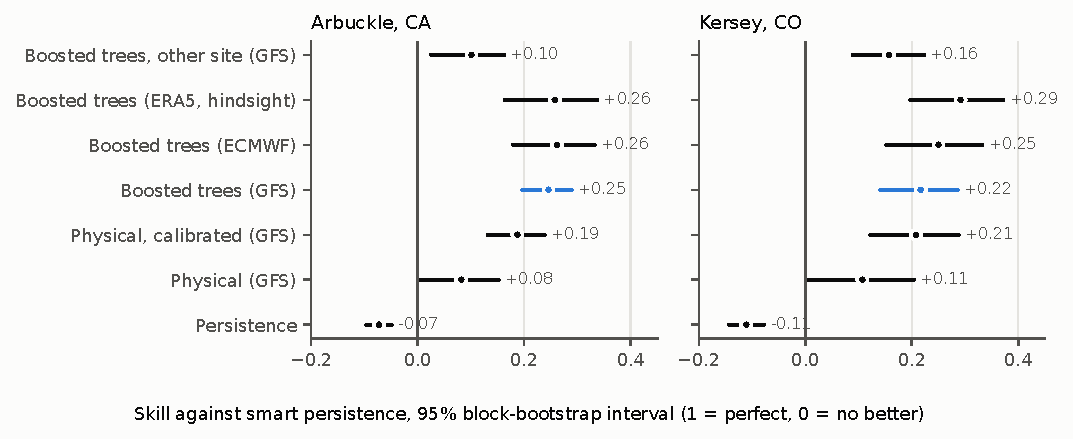
\includegraphics[width=\linewidth]{skill.pdf}
\caption{Skill against smart persistence with 95\% block-bootstrap intervals. The primary model is highlighted.}
\label{fig:skill}
\end{figure}

Boosted trees on the same GFS inputs reach \ArbGbmSkill\ (\ArbGbmLo\ to \ArbGbmHi) at Arbuckle and \KerGbmSkill\ (\KerGbmLo\ to \KerGbmHi) at Kersey. The question this study set out to answer is how much of that is the learning. Compared directly with the calibrated physical model on the same bootstrap blocks, the difference in RMSE (trees minus calibrated physical, as a fraction of rating) has a 95\% interval of \ArbGainLoGfs\ to \ArbGainHiGfs\ at Arbuckle, so there the trees are better. At Kersey the interval is \KerGainLoGfs\ to \KerGainHiGfs: no difference that this record can detect. Most of the skill, then, comes from a physical model and two fitted numbers; the trees add a modest amount at one site and nothing measurable at the other.

On the months both sites share (July 2024 to April 2025, \ArbDaysCommon\ and \KerDaysCommon\ days), smart persistence scores \ArbSmartNrmseCommon\ at Arbuckle and \KerSmartNrmseCommon\ at Kersey, and the trees' skill is \ArbGbmSkillCommon\ and \KerGbmSkillCommon. The ordering of the forecasters is the same as over the full period.

\subsection{Which weather}

Replacing GFS with the ECMWF forecast changes little at Arbuckle (trees \ArbGbmEcSkill) and helps at Kersey (\KerGbmEcSkill); the uncalibrated physical model gains more from ECMWF at both sites (\ArbPhysEcSkill\ and \KerPhysEcSkill), which suggests the GFS irradiance carries a bias the calibration and the trees mostly learn away. Giving the trees the weather that actually happened (ERA5) as if it had been forecast lifts skill only to \ArbGbmEraSkill\ at Arbuckle and \KerGbmEraSkill\ at Kersey. The day-ahead weather forecast is therefore not the main limit on these scores. At Arbuckle in particular, replacing the forecast with the reanalysis adds almost nothing; most of the remaining error is in how weather becomes power at this plant, in local conditions the reanalysis does not resolve either, and in the plant itself.

\subsection{Sky condition and season}

Figure~\ref{fig:sky} splits the errors by the day's measured clearness. On clear days, which are \ArbClearDays\ of \ArbDays\ at Arbuckle and \KerClearDays\ of \KerDays\ at Kersey, the trees' error is lowest (nRMSE \ArbClearGbmNrmse\ and \KerClearGbmNrmse) and their skill highest at Arbuckle (\ArbClearGbmSkill), likely because smart persistence is wrong on every clear day that follows a cloudy one and a weather forecast need not be. On overcast days errors are largest for every forecaster (trees \ArbOvercastGbmNrmse\ and \KerOvercastGbmNrmse) and skill is lowest (\ArbOvercastGbmSkill\ and \KerOvercastGbmSkill). At Kersey the calibrated physical model is as good as the trees on clear days (\KerClearPhysCalSkill\ against \KerClearGbmSkill); the trees' small advantage there is on mixed and overcast days.

\begin{figure}[t]
\centering
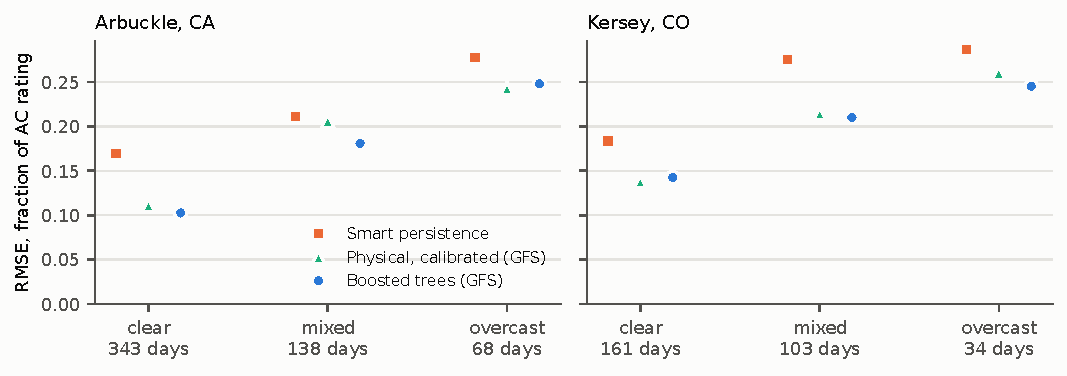
\includegraphics[width=\linewidth]{by_sky.pdf}
\caption{RMSE by the day's measured clearness (energy over clear-sky energy). Clear $\ge 0.8$, overcast $< 0.4$. The classes use the outcome and describe where error falls, not a forecastable state.}
\label{fig:sky}
\end{figure}

By season (Figure~\ref{fig:monthly}), Arbuckle's summers are easy for every forecaster: in June to August smart persistence scores \ArbJJASmartNrmse\ and the trees \ArbJJAGbmNrmse, a skill of only \ArbJJAGbmSkill. Winter is where forecasting pays: in December to February the same numbers are \ArbDJFSmartNrmse\ and \ArbDJFGbmNrmse, a skill of \ArbDJFGbmSkill. Kersey shows the same pattern with less contrast (summer \KerJJAGbmSkill, winter \KerDJFGbmSkill), and its smart persistence gets steadily worse through the winter and spring of 2025 while the weather-driven forecasts hold steady. Arbuckle's last months of 2025 stand out and are taken up in Section~\ref{sec:failures}.

\begin{figure}[t]
\centering
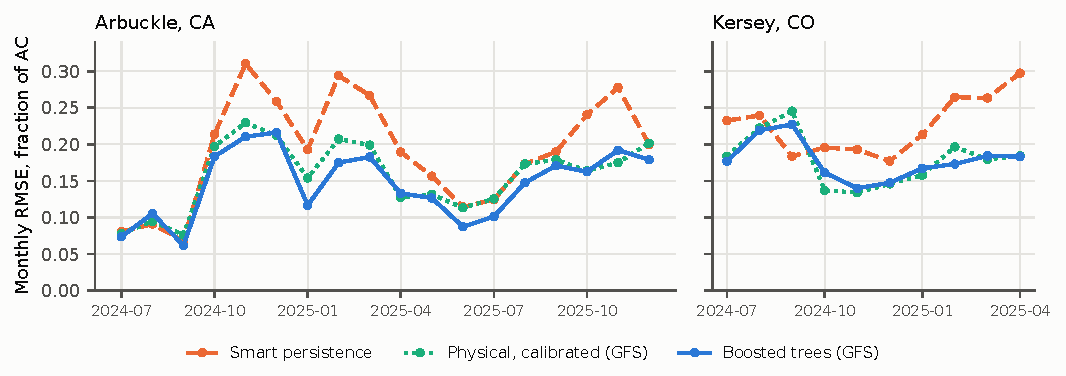
\includegraphics[width=\linewidth]{monthly.pdf}
\caption{Monthly RMSE for smart persistence, the calibrated physical model and the boosted trees (GFS inputs).}
\label{fig:monthly}
\end{figure}

\subsection{Transfer between sites}

A model trained only on the other plant, then given this plant's inputs, keeps a positive skill at both sites but loses much of it: \ArbTransferSkill\ (\ArbTransferLo\ to \ArbTransferHi) at Arbuckle and \KerTransferSkill\ (\KerTransferLo\ to \KerTransferHi) at Kersey, against \ArbGbmSkill\ and \KerGbmSkill\ when trained at home. The difference in RMSE, home model minus transferred model, has a 95\% interval of \ArbTransferGapLo\ to \ArbTransferGapHi\ of rating at Arbuckle and \KerTransferGapLo\ to \KerTransferGapHi\ at Kersey. Both models see physical and clear-sky power in units of each plant's own rating, so geometry and size are largely normalised away; what does not transfer is the relation between this site's weather forecasts and this plant's behaviour. That relation is, in a direct sense, ``about one place''. At both sites the transferred model's skill falls between that of the uncalibrated physical model (\ArbPhysSkill\ and \KerPhysSkill) and the calibrated one.

\subsection{Intervals}

The 10--90\% quantile band should hold 80\% of hours. It holds \ArbCovGfs\% at Arbuckle and \KerCovGfs\% at Kersey (mean width \ArbWidthGfs\ and \KerWidthGfs\ of rating; mean pinball loss \ArbPinballGfs\ and \KerPinballGfs). The bands are too narrow at both sites, and hindsight weather does not fix it (ERA5: \ArbCovEra\% and \KerCovEra\%). A likely reason is that quantile trees trained on a year or less learn the spread of errors in their training months, while the largest errors in the test months come from plant faults (described next) that no training month resembled.

\section{Failure analysis}\label{sec:failures}

Error is concentrated: the worst 10\% of days carry \ArbWorstTenAbs\% of all absolute error at Arbuckle and \KerWorstTenAbs\% at Kersey (\ArbWorstTenSq\% and \KerWorstTenSq\% of squared error). Of the scored days, \ArbDaysOverOne\ at Arbuckle and \KerDaysOverOne\ at Kersey were off by more than one rated hour of energy. Figure~\ref{fig:categories} sorts those days by the rules above.

\begin{figure}[t]
\centering
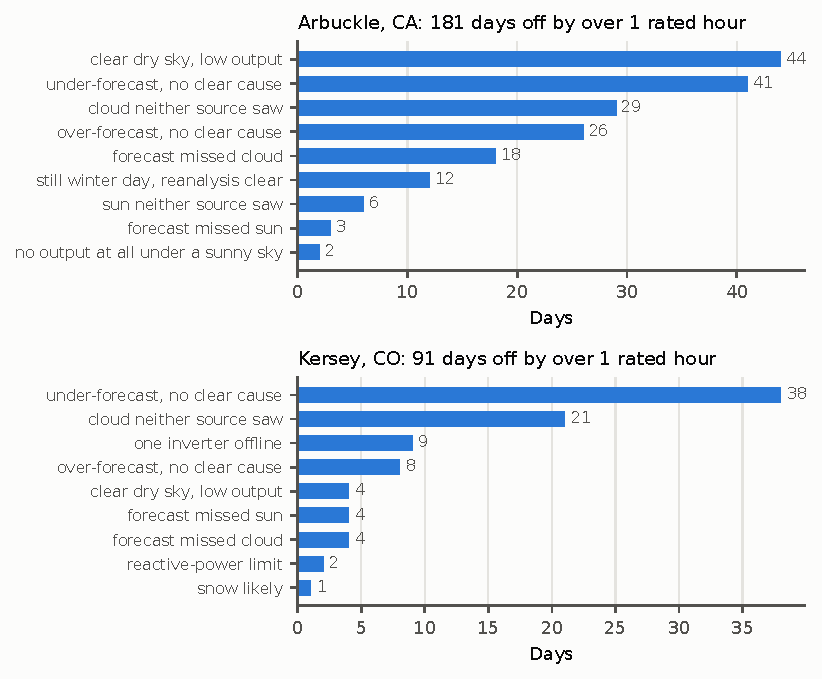
\includegraphics[width=0.85\linewidth]{categories.pdf}
\caption{Days with a daily energy error above one AC-rated hour, sorted by the fixed rules in \texttt{pipeline/failures.py}.}
\label{fig:categories}
\end{figure}

\paragraph{The plant, not the sky.} The single largest miss at Arbuckle is 18 October 2024: a clear day by the forecast and the reanalysis, and zero output all day (Figure~\ref{fig:cases}, top left). 6 November 2024 is the same. The data cannot say whether the plant was off or only its meter; either way, no weather forecast could have known. At Kersey, inverter~2 reported zero for days in mid-September 2024 while inverter~1's output was capped flat (top right); those days are five of Kersey's fifteen worst. From March 2025 Kersey's inverter~1 ran at a median power factor of \KerPfLate\ while producing, against \KerPfEarly\ before, consistent with a reactive-power setting; 1 April 2025 is the clearest case. At Arbuckle, \ArbCatClearDry\ days were clear and dry by both weather sources and the plant still made far less than clear-sky output (mean $k_\text{obs}$ \ArbCatClearDryKobs\ against $k_\text{era5}$ \ArbCatClearDryKera); almost all fall between May and September 2025. Equipment, soiling and wildfire smoke would all look like this in the data used here, and they cannot be separated without on-site measurements.

\paragraph{Still winter days.} \ArbCatStillWinter\ Arbuckle days in November to February had light wind, a reanalysis sky close to clear (mean $k_\text{era5}$ \ArbCatStillWinterKera), a day-ahead GFS forecast of partial cloud (mean $k_\text{nwp}$ \ArbCatStillWinterKnwp) and a plant that saw far less light than either (mean $k_\text{obs}$ \ArbCatStillWinterKobs). All of them fall in November and December 2025 (Figure~\ref{fig:cases}, bottom left). This pattern is consistent with radiation fog in the Sacramento Valley, a known winter phenomenon there \citep{baldocchi2014}, which a coarse model can miss. The data here do not prove it was fog. On these days the day-ahead forecast was closer to what happened than the reanalysis was.

\paragraph{Weather.} Only a minority of the large misses are a weather forecast that was wrong in a way the reanalysis later corrected: \ArbCatMissCloud\ days of missed cloud and \ArbCatMissSun\ of missed sun at Arbuckle, \KerCatMissCloud\ and \KerCatMissSun\ at Kersey. More common are days when both weather sources agreed and the plant saw something else: cloud that neither source saw (\ArbCatNeitherCloud\ and \KerCatNeitherCloud\ days). Kersey's 8 to 10 August 2024 (Figure~\ref{fig:cases}, bottom right) shows a different miss beside that one: on the 8th and 9th both weather sources called for heavy cloud and the trees still forecast several times the energy the plant made, so the error there is the model's, not the weather forecast's; on the 10th the plant saw cloud that neither source had. The largest single category at Kersey is under-forecasts with no clear cause (\KerCatUnderNone\ days): days that every source called clear (mean $k_\text{obs}$ \KerCatUnderNoneKobs, $k_\text{nwp}$ \KerCatUnderNoneKnwp, $k_\text{era5}$ \KerCatUnderNoneKera) on which the trees still predicted too little. Their cause was not investigated.

\begin{figure}[t]
\centering
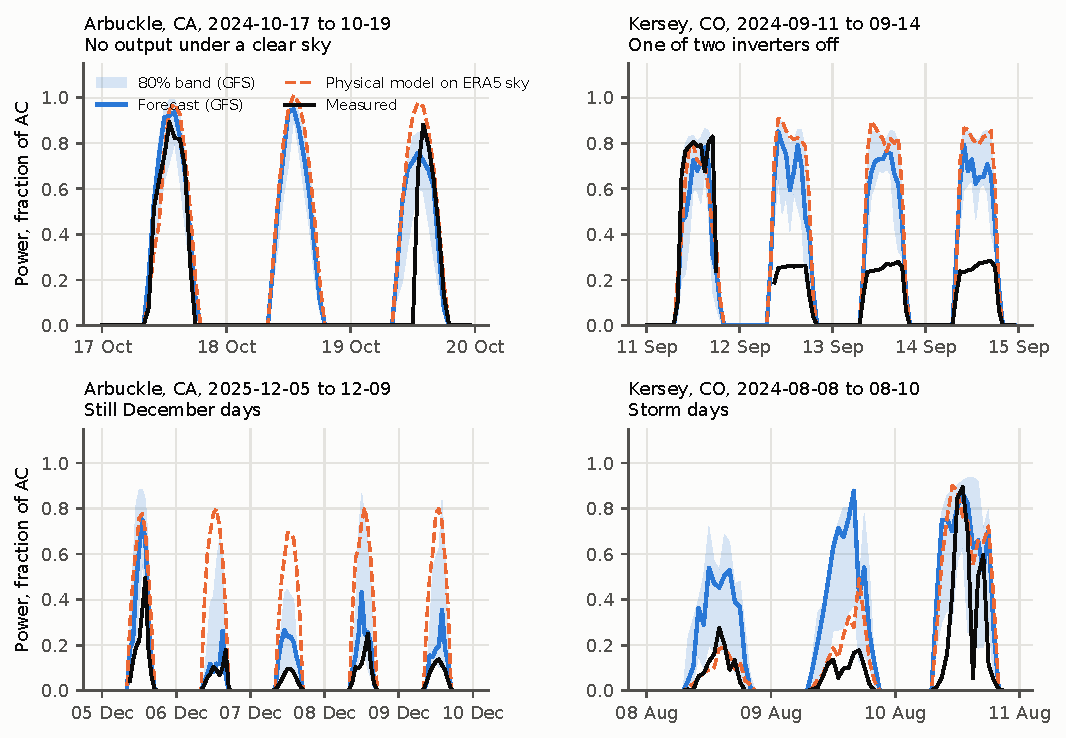
\includegraphics[width=\linewidth]{cases.pdf}
\caption{Four failure cases: measured power, the GFS-driven trees with their 80\% band, and the physical model on reanalysis (ERA5) weather.}
\label{fig:cases}
\end{figure}

\paragraph{How much the plant matters.} Removing the plant-anomaly days (\ArbAnomalyDays\ at Arbuckle, \KerAnomalyDays\ at Kersey; the rule uses no forecast) raises the trees' skill from \ArbGbmSkill\ to \ArbSensGbmSkill\ (\ArbSensGbmLo\ to \ArbSensGbmHi) at Arbuckle and from \KerGbmSkill\ to \KerSensGbmSkill\ (\KerSensGbmLo\ to \KerSensGbmHi) at Kersey. A forecast evaluated on a clean plant looks better than one evaluated on a real one, and the difference is about as large as the difference between the physical model and the trees.

\section{Limitations}

\begin{itemize}
\item Two plants. Neither is a cloudy humid site; the contrast is a Mediterranean valley against a semi-arid plain, because those were the plants with public data in the forecast archive's period. Kersey has 16 months, ten of them scored.
\item Short training records. The first test month has six months of history. Learned models, and especially the quantile bands, would likely improve with more years; this study cannot say by how much.
\item Hourly, single-point weather. Inputs are the hourly values at the nearest grid point. No spatial or ensemble information is used.
\item The plant faults are inferred from power, power factor and weather alone. Without maintenance logs, the categories ``no output'', ``clear dry sky, low output'' and ``still winter day'' are descriptions, not diagnoses.
\item Fixed, untuned hyperparameters. This avoids optimism, but a tuned model might do somewhat better.
\item The Open-Meteo archive is a third-party reconstruction of past runs. The pipeline pins dates and records a checksum of every response, but cannot rule out later changes to the archive.
\end{itemize}

\section{Reproducibility}

Everything runs from one command, \texttt{python -m pipeline all}: it downloads the raw files (about 30\,MB) and checks them against the committed SHA-256 manifest, cleans the series and writes the ledger, builds the features, runs the rolling-origin evaluation, sorts the failures, draws the figures and writes the macros this paper's numbers are typeset from. A full run takes a few minutes on a laptop. Seeds are fixed and LightGBM runs single-threaded in deterministic mode; a rerun from an empty data folder reproduced every committed result file exactly. Unit tests cover the cleaning rules and metrics, and an end-to-end test on a synthetic plant checks that the pipeline ranks hindsight weather above the forecast and both above smart persistence and that a planted leak is caught. The code is MIT-licensed at \url{https://github.com/speyyman/solar-two-sites}; this text and its figures are CC BY 4.0. Data sources and licences are listed in the repository's \texttt{DATA.md}.

\section*{Acknowledgements}

Measured plant data are from the NREL PVDAQ archive on the Open Energy Data Initiative. Weather data are from Open-Meteo, which redistributes NOAA GFS, ECMWF IFS open data and Copernicus ERA5. The author thanks the maintainers of pvlib, LightGBM and the scientific Python stack.

\textbf{AI assistance.} The analysis code and the drafting of this paper were done with Claude (Anthropic), an AI assistant, under the author's direction. The author is responsible for the content.

\bibliographystyle{plainnat}
\bibliography{references}

\appendix
\section{Cleaning ledger}\label{app:ledger}

Every value the pipeline dropped, shifted or filled in, by rule. ``Power'' rows are the measured output used for every score; ``POA'' rows are the on-site irradiance sensors, which were checked but not used; ``features'' rows are fills in the persistence inputs.

\begin{center}
\scriptsize
% Generated by pipeline/report.py. Do not edit.
\begin{tabular}{llrl}
\toprule
Site & Rule & Count & Unit \\
\midrule
Arbuckle & timestamp ambiguous or nonexistent in local clock; dropped & 4 & samples \\
Arbuckle & timestamp ambiguous or nonexistent in local clock; dropped & 8 & samples \\
Arbuckle & overlapping timestamps across files; first file kept & 29,175 & samples \\
Arbuckle & clock shifted to match solar noon & 70,159 & samples \\
Arbuckle & negative power (night tare) set to 0 & 0 & samples \\
Arbuckle & above 105\% of maximum AC output; dropped & 0 & samples \\
Arbuckle & identical non-zero value for 60 min or more; dropped & 153 & samples \\
Arbuckle & hour with under 75\% of its samples; set missing & 32 & hours \\
Arbuckle & clock shifted to match solar noon & 73,077 & samples \\
Arbuckle & month whose clock disagrees with the sun by more than 0.75 h; dropped & 2,898 & samples \\
Arbuckle & month whose clock disagrees with the sun by more than 0.75 h; dropped & 2,893 & samples \\
Arbuckle & overlapping timestamps across files; first file kept & 54,253 & samples \\
Arbuckle & hour with under 75\% of its samples; set missing & 9,001 & hours \\
Kersey & sample missing in source & 1,458 & samples \\
Kersey & timestamp ambiguous or nonexistent in local clock; dropped & 12 & samples \\
Kersey & negative power (night tare) set to 0 & 1,561 & samples \\
Kersey & above 105\% of maximum AC output; dropped & 0 & samples \\
Kersey & identical non-zero value for 60 min or more; dropped & 0 & samples \\
Kersey & hour with under 75\% of its samples; set missing & 52 & hours \\
Kersey & timestamp ambiguous or nonexistent in local clock; dropped & 7 & samples \\
Kersey & clock shifted to match solar noon & 137,153 & samples \\
Kersey & month whose clock disagrees with the sun by more than 0.75 h; dropped & 8,791 & samples \\
Kersey & hour with under 75\% of its samples; set missing & 32 & hours \\
Arbuckle & smart persistence: D-1 incomplete, ratio taken from an older day & 31 & days \\
Arbuckle & persistence: D-1 missing, filled from an older day (up to 7) & 52 & day-hours \\
Kersey & smart persistence: D-1 incomplete, ratio taken from an older day & 36 & days \\
Kersey & persistence: D-1 missing, filled from an older day (up to 7) & 351 & day-hours \\
\bottomrule
\end{tabular}

\end{center}

\end{document}
